\documentclass[10pt,a4paper]{article}

\usepackage[latin1]{inputenc}
\usepackage{amsmath}
\usepackage{amsfonts}
\usepackage{amssymb}
\usepackage{graphicx}
\usepackage{listings}
\title{Assignment No :B7}
\date{}
\author{Roll No.4431}


\begin{document}
\maketitle
\section{Title:}
Odd-Even Merge Sort

\section{Problem Definition}
Perform concurrent Odd-Even Merge sort using HPC infrastructure (preferably BBB) using Python/Scala/ Java/ C++.

\section{Learning Objectives}
\begin{enumerate}
\item To understand the concept of Algorithmic problem solving and using it for sorting.
\item To understand the Odd-Even merge sort algorithm..
\end{enumerate}

\section{Learning Outcomes}
\begin{enumerate}
\item Ability to analyse the problems and solve them using problem solving techniques.
\item Acquire proficiency over the programming language of choice and induce HPC based infrastructure in them.
\end{enumerate}


\section{Related Mathematics}
Let S be the solution perspective of the given problem.
\\\\The set S is defined as:
\\\\$S=\lbrace\ s,e,X,Y,F,DD,NDD,S_{c},F_{c}|\varnothing_{s}\rbrace$
\\\\Where,
\\\\s= Start state,  Such that $Y=\lbrace \varnothing \rbrace$ 
\\\\e= End state 
\\\\X= Input Set.
\\\\$X=\lbrace$ $seq(x)$ $\mid$ $x_i \in Natural Numbers$ $\rbrace$
\\\\Y=Output set.
\\\\$Y=\lbrace $ sorted input sequence $ \rbrace $
\\\\F= Set of functions used.
\\\\F=$\lbrace getData(), sortData(), putData() \rbrace$
\\\\getData() = function to get the elements for sorting.
\\\\sortData()= function to sort the input sequence using the Odd-Even Merge sort algorithm.
\\\\getData() = function to display the result of the sorting.
\\\\DD=Deterministic data.
\\DD=
\begin{enumerate}
\item elements of the input sequence are proper.
\item solution is defined and exists.
\item computation as well as the input sequence terminates.
\end{enumerate}
NDD= Non-deterministic data.
\\NDD= $\cup$ - DD


\section{State Transition diagram}
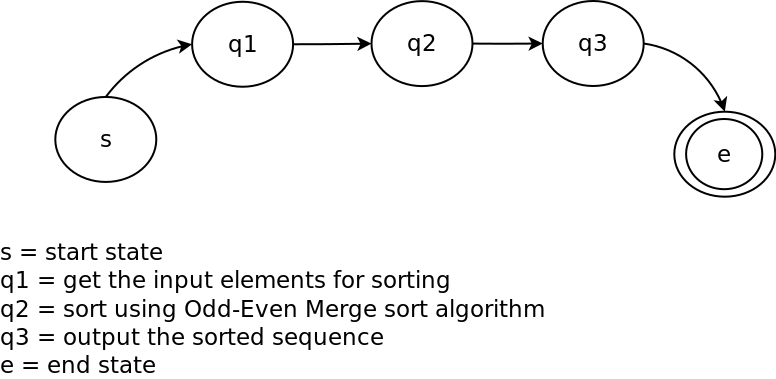
\includegraphics[scale=0.5]{stdg.png}

\section{Concepts related theory}
\subsection{Odd-Even Merge Sort} 
	Odd-even sort is a relatively simple sorting algorithm, developed originally for use on parallel processors with local interconnections. It is a comparison sort related to bubble sort, with which it shares many characteristics. It functions by comparing all odd/even indexed pairs of adjacent elements in the list and, if a pair is in the wrong order (the first is larger than the second) the elements are switched. The next step repeats this for even/odd indexed pairs (of adjacent elements). Then it alternates between odd/even and even/odd steps until the list is sorted.
	
	\subsection{Merge Sort}
	Merge sort (also commonly spelled mergesort) is an efficient, general-purpose, comparison -based sorting algorithm. Most implementations produce a stable sort, which means that the implementation preserves the input order of equal elements in the sorted output. Mergesort is a divide and conquer algorithm that was invented by John von Neumann in 1945.  
	
	\subsection{Example}
	Merging the two lists a1,a2,...,an and b1,b2,...,bn, where n is a power of 2. 
	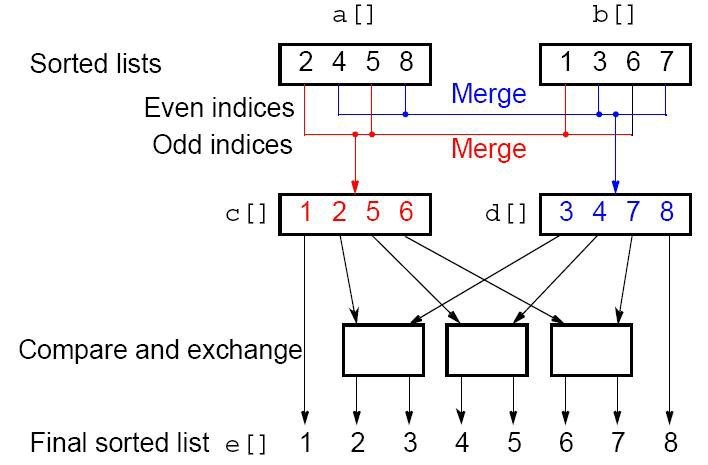
\includegraphics[width=\textwidth]{oddeven_example}
		
	\subsection{Beaglebone Black}
	\textbf{BeagleBone Black Overview:}\\ 
	The BeagleBone Black is the latest addition to the BeagleBoard.org family and like its predecessors, is designed to address the Open Source Community, early adopters, and anyone interested in a low cost ARM Cortex-A8 based processor. It has been equipped with a minimum set of features to allow the user to experience the power of the processor and is not intended as a full development platform as many of the features and interfaces supplied by the processor are not accessible from the Beagle Bone Black via on board support of some interfaces. It is not a complete product designed to do any particular function. It is a foundation for experimentation and learning how to program the processor and to access the peripherals by the creation of your own software and hardware. It also offers access to many of the interfaces and allows for the use of add-on boards called capes, to add many different combinations of features. A user may also develop their own board or add their own circuitry.
	
	\textbf{Board Component Locations:}\\ 
	This section describes the key components on the board. It provides information on their location and function. Familiarize yourself with the various components on the board. 
	\begin{itemize}
		\item Connectors, LEDs, and Switches 
		\item DC Power is the main DC input that accepts 5V power. 
		\item Power Button alerts the processor to initiate the power down sequence.  
		\item 10/100 Ethernet is the connection to the LAN. 
		\item Serial Debug is the serial debug port. 
		\item USB Client is a mini USB connection to a PC that can also power the board. 
		\item BOOT switch can be used to force a boot from the SD card. 
		\item There are four blue LEDS that can be used by the user. 
		\item Reset Button allows the user to reset the processor. 
		\item uSD slot is where a uSD card can be installed. 
		\item microHDMI connector is where the display is connected to. 
		\item USB Host can be connected different USB interfaces such asWi-Fi, BT,Keyboard, etc  	
	\end{itemize}
	
	\textbf{Features of Beaglebone Black}\\
	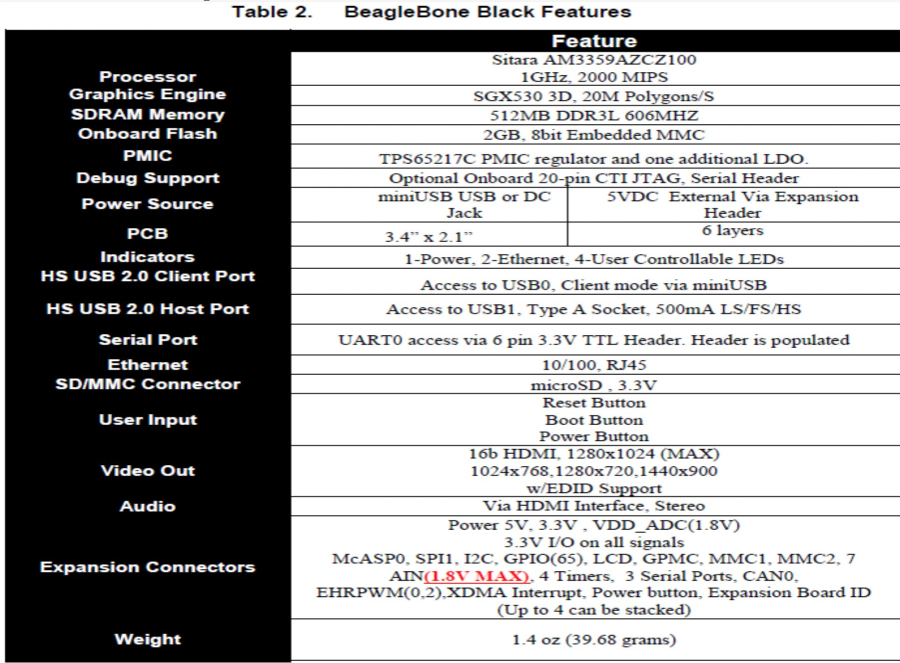
\includegraphics[width=\textwidth]{features_bbb.png}
	
	\textbf{Key Components}
	\begin{itemize}
		\item Sitara AM3359AZCZ100 is the processor for the board. 
		\item Micron 512MB DDR3L is the Dual Data Rate RAM memory. 
		\item TPS65217C PMIC provides the power rails to the various components on the board. 
		\item SMSC Ethernet PHY is the physical interface to the network. 
		\item Micron eMMC is an onboard MMC chip that holds up to 2GB of data. 
		\item HDMI Framer provides control for an HDMI or DVI-D display with an adapter. 
	\end{itemize}
	\vspace{30px}
	
	
	\textbf{Connectivity}
	\begin{itemize}
		\item Connect the small connector on the USB cable to the board as shown in Figure 1. The connector is on the bottom side of the board. 
		\item Connect the large connector of the USB cable to your PC or laptop USB port. 
		\item The board will power on and the power LED will be on as shown in Figure 2 below. 
	\end{itemize}
	
	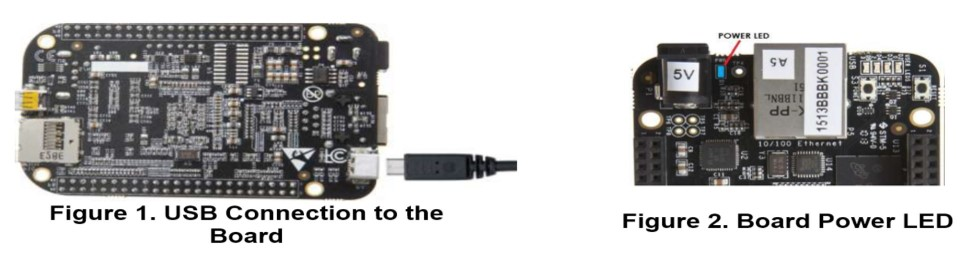
\includegraphics[width=\textwidth]{bbb_01}
	
	\begin{itemize}
		\item Apply Power: 
		The final step is to plug in the DC power supply to the DC power jack as shown in Figure4 below. 
		
		\item Booting the Board: 
		As soon as the power is applied to the board, it will start the booting up process. When the board starts to boot the LEDs will come on in sequence as shown in Figure 5 below. It will take a few seconds for the status LEDs to come on, so be patient. The LEDs will be flashing in an erratic manner as it boots the Linux kernel. 
	\end{itemize}
	
	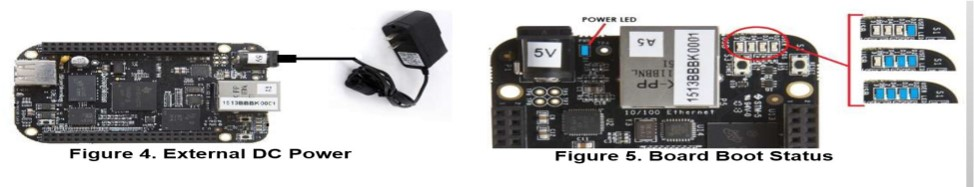
\includegraphics[width=\textwidth]{bbb_02}
	
	\subsection{Steps to run program in Beaglebone Black}
	1.	In red hat terminal we need to type following command for accessing the beagle bone terminal. 
	ssh 192.168.7.2 \\
	2.	Open another redhat terminal for copying the python program from redhat to beagle bone by using command: 
	scp filename.py root@192.168.7.2: \\
	3.	Now open beagle bone terminal to check whether program is copied or not by using command ls. \\
	4.	To run the program write following command in beagle bone terminal. 
	python filename.cpp \\
	
	\subsection{Odd-Even Merge Sort}
	template <class T> 									\\
	void OddEvenSort (T a[], int n) 					\\
	{ for (int i = 0 ; i < n ; i++) 					\\
		{ if (i \& 1) // 'i' is odd 					\\
			{ for (int j = 2 ; j < n ; j += 2) 			\\
				{ if (a[j] < a[j-1]) swap (a[j-			\\
					1], a[j]) ; 						\\
				} 										\\
			} else 										\\
			{ 											\\
				for (int j = 1 ; j < n ; j += 2) { 		\\
					if (a[j] < a[j-1]) 					\\
					swap (a[j-1], a[j]) ; 				\\
				} 										\\
			} 											\\
		} 												\\
	} 													\\
														\\
	
	\subsection{Merge Sort}
	function merge\_sort(node head) 								\\ 
	if (head == nil)  	return nil 								\\
	var node array[32]; initially all nil var 					\\
	node result 												\\
	var node next var int i result = head						\\ 
	// merge nodes into array while 							\\
	(result != nil) next = result.next;  	result.next = nil 	\\
	for(i = 0; (i < 32) \&\& (array[i] != nil); i += 1) 		\\
	result = merge(array[i], result) 							\\
	array[i] = nil 												\\
	// do not go past end of array if (i == 32)					\\ 
	i -= 1 array[i] = result 									\\
	result = next 												\\
	// merge array into single list								\\ 
	result = nil 												\\
	for (i = 0; i < 32; i += 1) 								\\
		result = merge(array[i], result) 						\\
	return 														\\
	result 														\\
	
	\subsection{Parallel Odd Even Sort}
	void ODD-EVEN-PAR(n) 										\\
	{ 															\\
		id = process label 										\\
		for (i= 1; i<= n; i++) 									\\
		{ 														\\
			if (i is odd) 										\\
				compare-and-exchangemin(id+1);					\\
			else												\\
				compare-and-exchangemax(id-1);					\\
			if (i is even)										\\
				compare-andexchange-min(id+1); 					\\
			else 												\\
				compare-and-exchange-max(id-1); 				\\
		} 														\\
	}															\\

	\subsection{Complexity}
		O(log2n)

\section{Program Listing}
\begin{lstlisting}
#include<iostream>
#include<omp.h>

using namespace std;

//function for swap
void swap(int *a,int* b)
{
  int temp;
  temp=*a;
  *a=*b;
  *b=temp;
}

//print array
void printArr(int *arr,int size,int val)
{
	cout<<"\n after iteration "<<val<<" \n";
	for(int i=0;i<size;i++)
	cout<<arr[i]<<"\t";
	cout<<endl;
}


//odd_even sort function
void odd_even(int * arr,int size)
{
	int tid;
	int k=0;

	omp_set_num_threads(size/2);
	while(k<size)
	{
		if(k%2 == 0)
		{	
			#pragma omp parallel for	
			//for even iteration
			for(int i=0;i<size;i+=2)
			{
			   tid = omp_get_thread_num();
			  cout <<"\ncurrent thread no :"<<tid;
			  if(i!=size-1)
			  if(arr[i] > arr[i+1])	
			  swap( (arr+i), (arr+i+1));
			}
		}
		else
		{
			#pragma omp parallel for
			//for odd iteration
			for(int j=1;j<size;j+=2)
			{
			 	 tid = omp_get_thread_num();
				 cout <<"\ncurrent thread no :"<<tid;
				//skip for last iteration
			 	if(j!=size-1)
				 if(arr[j] > arr[j+1])
				
				 swap((arr+j),(arr+j+1));
			}
		}
		//print array
		printArr(arr,size,k);
		k++;
	}
}

int main()
{
	int size=0;
	cout<<"enter the array size";
	cin>>size;
	
	int *arr = new int[size];
	
	cout<<"\nenter array elements";
	for(int i=0;i<size;i++)
	cin>>arr[i];
 	
	odd_even(arr,size);
	
return 0;
}
\end{lstlisting}


\section{Output}
\begin{lstlisting}
botman@botmatrix:~/Programming/College/CL4-master/HPC/B7_HPC_Odd-Even$ g++ 
B6.cpp -o OUT -fopenmp
botman@botmatrix:~/Programming/College/CL4-master/HPC/B7_HPC_Odd-Even$ ./OUT
enter the array size 5

enter array elements 5 4 3 2 1

current thread no :
current thread no :00
current thread no :0
 after iteration 0 
4	5	2	3	1	

current thread no :0
current thread no :0
 after iteration 1 
4	2	5	1	3	

current thread no :0
current thread no :0
current thread no :0
 after iteration 2 
2	4	1	5	3	

current thread no :0
current thread no :0
 after iteration 3 
2	1	4	3	5	

current thread no :0
current thread no :
current thread no :00
 after iteration 4 
1	2	3	4	5	
botman@botmatrix:~/Programming/College/CL4-master/HPC/B7_HPC_Odd-Even$ 


\end{lstlisting}

\section{TESTING :}
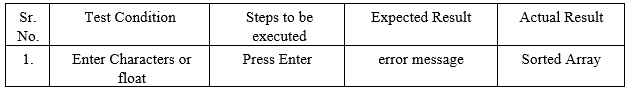
\includegraphics[width=\textwidth]{oddeven_negative}
			
\section{CONCLUSION : }
	From this assignment we have studied concept of Odd-Even Merge sort and developed time and space efficient algorithm using multicore, concurrent environment. 

\end{document}